\documentclass{article}
\usepackage{fullpage}
\usepackage{blindtext}
\usepackage[T1]{fontenc}
\usepackage[utf8]{inputenc}
\usepackage{subcaption}
\usepackage{amsmath, amssymb, amsthm, mathtools}
\DeclarePairedDelimiter\bra{\langle}{\rvert}
\DeclarePairedDelimiter\ket{\lvert}{\rangle}
\DeclarePairedDelimiterX\braket[2]{\langle}{\rangle}{#1 \delimsize\vert #2}
\setlength\parindent{0pt}
\usepackage{titlesec}
\usepackage{siunitx}
\usepackage{enumitem}
\newcommand{\uvec}[1]{\boldsymbol{\hat{\textbf{#1}}}}
\usepackage{graphicx}
\graphicspath{ {./images/} }
\usepackage{color}   
\usepackage{hyperref}
\usepackage{physics}
\usepackage{enumitem}
\usepackage{comment}
\usepackage[nodisplayskipstretch]{setspace}
\hypersetup{
    colorlinks=true,
    linkcolor=green,
    filecolor=magenta,      
    urlcolor=cyan,
}

\title{CTA200 2021 Assignment 2}
\author{Alex Laroche}
\date{\today}

\begin{document}

\maketitle

\begin{enumerate}

\item The errors for each derivative method are shown below.
\begin{figure}[htb!]
    \centering
    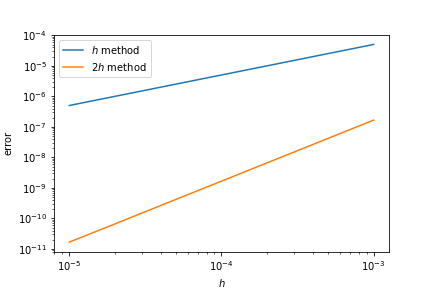
\includegraphics[scale=0.7]{deriv_err.png}
    \caption{Derivative errors}
    \label{fig:deriv}
\end{figure}

We observe that the second method is indeed better since the errors are several orders of magnitude lower. The slopes of both curves demonstrate the need for $h$ to be small. As $h$ increases, the numerical derivatives become progressively worse estimations of the analytic derivative. Hence, the slope of the error curves are positive.

\newpage

\item First, we plot the Mandelbrot set with a binary convergent/divergent color map. We then plot the Mandelbrot set with a multicoloured scale depending on the rate of convergence.
\begin{figure}[htb!]
\begin{subfigure}{.5\textwidth}
  \centering
  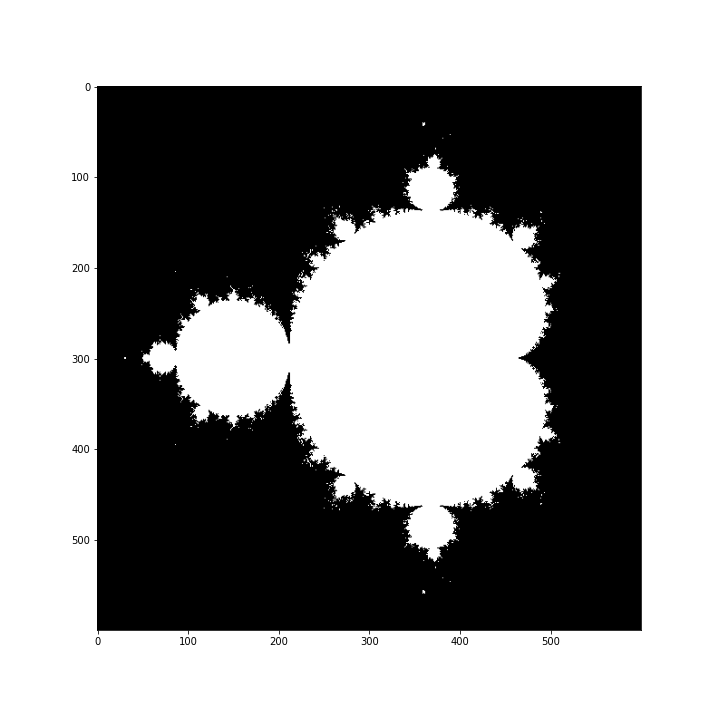
\includegraphics[width=.8\linewidth]{mandelbrot_binary.png}
  \caption{Binary map}
  \label{fig:sfig1}
\end{subfigure}%
\begin{subfigure}{.5\textwidth}
  \centering
  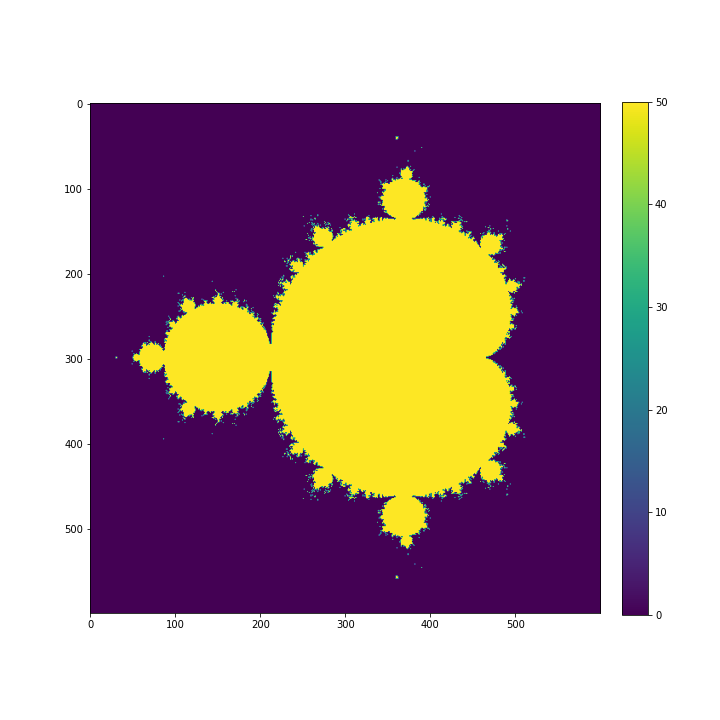
\includegraphics[width=.8\linewidth]{mandelbrot_multi.png}
  \caption{Multicoloured map.}
  \label{fig:sfig2}
\end{subfigure}
\label{fig:fig}
\end{figure}

The white region on the left corresponds to the Mandelbrot set; the region of the complex plane which is convergent for the iterative equation $z_{i+1}=z_i^2+c,$ for $c\in\mathbb{C}.$ The black region is divergent. On the right, we observe that near the convergent/divergent boundary, the function diverges at varying rates. As we move outward, the divergence becomes more extreme. The detail of the right plot is evidently poor in comparison to typical Mandelbrot images. Increasing resolution could resolve this.

\newpage

\item SIR model solutions for three $\gamma,\beta$ pairs are shown below.
\begin{figure}[htb!]
    \centering
    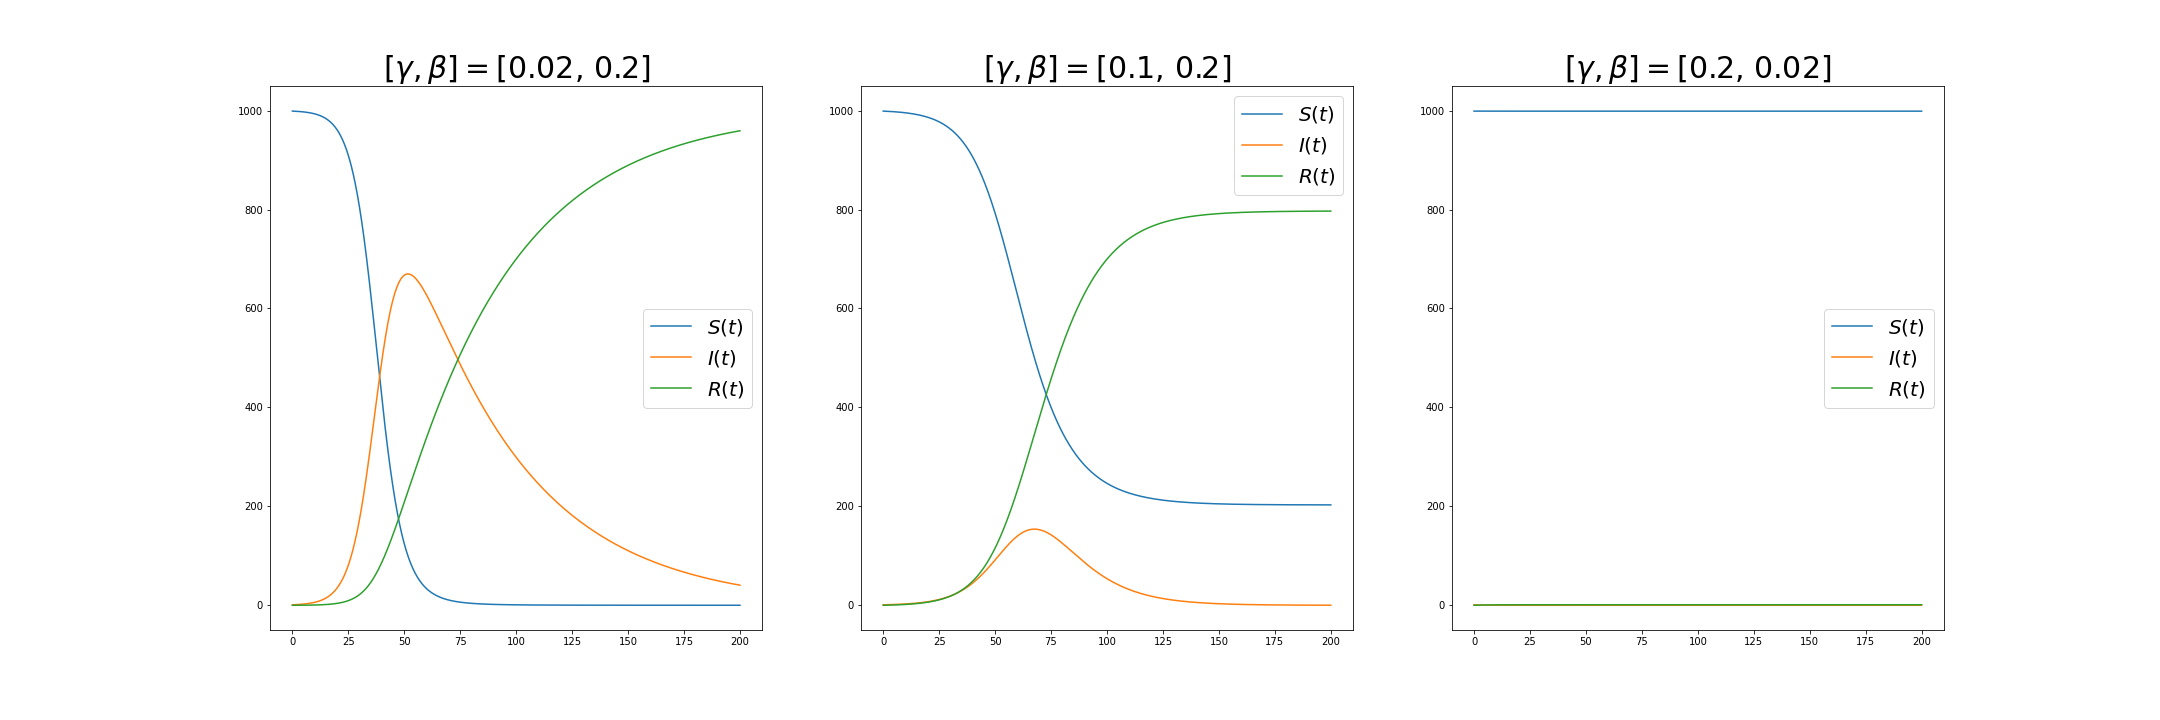
\includegraphics[scale=0.23]{SIR.png}
    \caption{Susceptible, infectious and recovered curves as functionfs of time.}
    \label{fig:my_label}
\end{figure}
Depending on the ratio $R_0=\beta/\gamma,$ the basic reproduction ratio, different scenarios can occur. On the left, if $R_0\gg1,$ we observe that the disease will quickly spread to infect the entire population. Given infinite time, the entire population will recover since the recovered are asymptoting to $R=N$ and the infected are asymptoting to $I=0.$ In the center, if $R_0=O(1),$ some of the population will remain susceptible since the disease cannot spread quickly enough to infect the entire population. On the right, a scenario in which $R_0\ll 1$ is depicted. In this case, no spread occurs since the disease is not infectious enough to propagate through the population.
    
\end{enumerate}



\end{document}
